\chapter{Loudspeaker Analysis}
\label{chapter:LoudspeakerAnalysis}

\section{Introduction}
A speaker functions by converting electrical current into mechanical motion, thereby generating an acoustic signal. The current passing through the voice coil induces vibrations in the speaker cone, causing a difference in sound pressure and thus producing sound waves. The speaker's physical dimensions are crucial in shaping its response to electrical inputs. To design efficient filters, it is necessary to represent the speaker's behavior with an equivalent electrical circuit. This approach facilitates precise predictions of the speaker's response to different input signals. This chapter outlines the structure of the electrical model and the methodologies used to determine its parameters.

\subsection{Loudspeaker Specifications}
The objective is to determine the appropriate values for the capacitors, inductors, and resistors in the electrical equivalent circuit representing the physical loudspeakers. Once these component values are identified, the circuit will be simulated over the frequency range of 20Hz to 20kHz. The simulated behavior will then be compared with the measured frequency response of the loudspeakers, ensuring that any significant deviation and discrepancy between the measured and simulated responses remains minimal to ensure high efficiency and function as projected.

\section{Loudspeaker Circuit Models}
\subsection{Model at Resonant Frequency}
The behavior of the speakers can be represented by an equivalent circuit comprising resistors, capacitors, and inductors. The capacitors and inductors model the speaker's frequency-dependant characteristics. At certain frequencies, the speaker exhibits predominantly higher resistive behavior, primarily influenced by the natural resonant frequency of the speaker's cone. The circuit model consists of five elements arranged as shown in Fig. \ref{fig:impedance_model1}. Here, $R_e$ represents the impedance at DC conditions, $L_e$ models the inductance of the voice coil, and the parallel RLC branch represents the mechanical properties of the cone. In this parallel branch, $R_p$ corresponds to frictional losses, $L_p$ models the mass of the cone, and $C_p$ represents its spring-like behavior \cite{johnshopkins_rlc}.
\begin{figure}[H]
    \centering
    \captionsetup{justification=raggedright, labelfont=bf}
    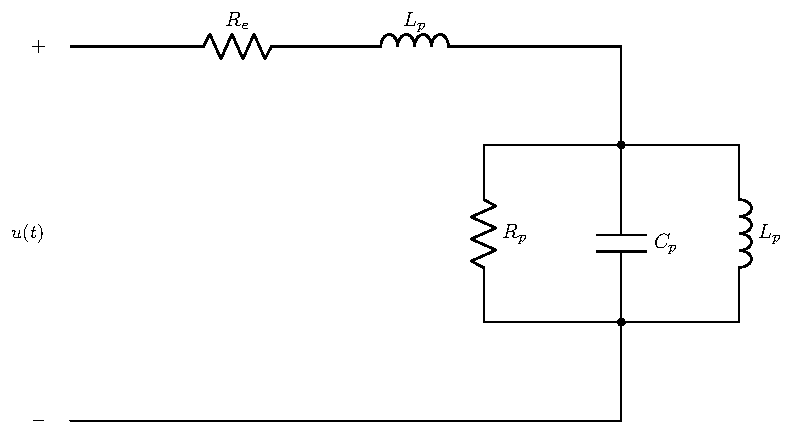
\includegraphics[width=0.6\linewidth]{figures/FilterGroup/ImpedanceModel1.pdf}
    \caption{Impedance model of the loudspeakers, depicting the equivalent circuit configuration used to represent the speaker's electrical ($R_e$, $L_e$) and mechanical properties ($R_p$, $C_p$, $L_p$ )\cite{IP-manual}.}
    \label{fig:impedance_model1}  
\end{figure}

\subsection{Model above Resonant Frequency}
At frequencies above and significantly higher than the cone's resonant frequency, the equivalent circuit can be further simplified. The total impedance of the circuit could be calculated using Eq. \ref{eq:total impedance}. For $\omega \gg \omega_o$, where $\omega_o$ is the resonant frequency of the circuit, the parallel components $R_p, C_p$ and $L_p$ can be disregarded due to their diminished influence on the overall impedance. To justify this simplification, the analysis should employ a normalized angular frequency $\omega'$ defined as followed:
\begin{flalign}
    \label{eq:normalize frequency}
    \omega' = \frac{\omega}{\omega_o}
    \equnit{\si{\text{rad s^{-1}}}}
\end{flalign}
The total impedance of the loudspeaker model is given by
\begin{flalign}
    \label{eq:total impedance}
    Z_{tot} = R_e + j\omega L_e + \frac{1}{\frac{1}{R_p}+j\omega C_p+\frac{1}{j\omega L_p}}
    \equnit{\si{\Omega}}
\end{flalign}

By applying Eq. \ref{eq:normalize frequency} and substituting it into Eq. \ref{eq:total impedance}, a revised expression for the total impedance, $Z_{tot}$, is obtained, as presented in Eq. \ref{eq:normalized impedance}:
\begin{flalign}
    \label{eq:normalized impedance}
    Z_{tot} = R_e + j\frac{\omega'}{\sqrt{L_pC_p}}L_e + \frac{1}{\frac{1}{R_p}+j\sqrt{\frac{C_p}{L_p}}\left(\omega'-\frac{1}{\omega'}\right)}
    \equnit{\si{\Omega}}
\end{flalign}

%-----------------------------------------------------------

You can rewrite $\omega$ as $\omega'\omega_o$. We can substitute the expression from Eq~\ref{eq:resonant frequency appA} \cite{IP-manual} and we will end up with the final expression for $\omega$ as seen in Eq~\ref{eq:final omega appA}.

\begin{flalign}
    \label{eq:resonant frequency appA}
    \omega_o = \frac{1}{\sqrt{L_pC_p}}
    \equnit{\si{\text{rad s^{-1}}}}
\end{flalign}

\begin{flalign}
    \label{eq:final omega appA}
    \omega = \frac{\omega'}{\sqrt{L_pC_p}}
    \equnit{\si{\text{rad s^{-1}}}}
\end{flalign}

For the next part I would like to define $Z_{par}$ as the impedance of the parallel RCL part of the circuit (Eq~\ref{eq:parallel impedance appA}).
\begin{flalign}
    \label{eq:parallel impedance appA}
    Z_{par} = \frac{1}{\frac{1}{R_p}+j\omega C_p+\frac{1}{j\omega L_p}}
    \equnit{\si{\Omega}}
\end{flalign}

If we want have a look at what happens with $Z_{par}$ when $\omega >> \omega_o$, we could see what happens to the impedance when $\omega'>>1$. First we need to rewrite the equation in terms of $\omega'$:
\begin{flalign}
\label{eq:capacitive_impedance appA}
    j\omega C_p = j\omega'\sqrt{\frac{c_p}{L_p}}
    \equnit{\si{\Omega^{-1}}}
\end{flalign}
\begin{flalign}
\label{eq:inductive_impedance appA}
    \frac{1}{j\omega L_p} = -j\frac{1}{\omega'}\sqrt{\frac{C_p}{L_p}}
    \equnit{\si{\Omega^{-1}}}
\end{flalign}

Substituting Eq~\ref{eq:capacitive_impedance appA} and Eq~\ref{eq:inductive_impedance appA} into Eq~\ref{eq:parallel impedance appA} will result in Eq~\ref{eq:normalized impedance appA}.

\begin{flalign}
    \label{eq:normalized impedance appA}
    Z_{par} = \frac{1}{\frac{1}{R_p}+j\sqrt{\frac{C_p}{L_p}}(\omega'-\frac{1}{\omega'})}
    \equnit{\si{\Omega}}
\end{flalign}

Now we can observe that if $\omega'>>1$ then $Z_{par} << 1$. Because $Z_{tot} = R_e + j\omega L_p + Z_{par}$ we can say that if $\omega >> \omega_o$ then $Z_{tot} \approx R_e + j\omega L_p$.

%---------------------------------------------------------

The revised expression for $Z_{tot}$ corresponds to an equivalent circuit consisting of an inductor and a resistor, as shown in Fig \ref{fig:impedance_model2}. If the operating frequencies of the speaker are all significantly higher than the resonant frequency, utilizing this simplified model becomes more practical for analysis and design purposes.
\begin{figure}[H]
    \centering
    \captionsetup{justification=raggedright, labelfont=bf}
    \includegraphics[width=0.5\linewidth]{figures/FilterGroup/impedance_model2_speaker.jpg}
    \caption{Impedance model for frequencies above the resonant frequency, illustrating the simplified equivalent circuit consisting of an inductor $L_e$ and the resistor $R_e$ \cite{IP-manual}.}
    \label{fig:impedance_model2}
\end{figure}

\section{Calculate Model Parameters}
The determination of the five unknown parameters requires solving a set of five equations. By analyzing the circuit and its impedance, the necessary equations for parameter estimation can be derived. The measured impedance data is presented in Fig \ref{fig:abs_speakers}. Detailed derivations of these equations are provided in the IP-manual \cite{IP-manual}.
\begin{flalign}
    \label{eq:Re_model}
    R_e = \left. |Z| \right._{\omega=0}
    \equnit{\si{\Omega}}
\end{flalign}

where $R_e$ represents the equivalent resistance of the circuit under DC conditions, corresponding to the impedance when the frequency is zero ($\omega=0$). Similarly, the parallel resistance $R_p$ is derived by subtracting $R_e$ from the magnitude of the total impedance $|Z|$ at the resonant angular frequency denoted by $\omega= \omega_o$, as given in Eq. \ref{eq:Rp_model}:
\begin{flalign}
    \label{eq:Rp_model}
    R_p = \left. |Z| \right._{\omega=\omega_o} - R_e
    \equnit{\si{\Omega}}
\end{flalign}

where $R_p$ accounts for the frictional losses in the mechanical behavior of the speaker at resonance. The capacitance $C_p$, representing the spring behavior of the speaker cone, is related to $R_p$ by Eq. \ref{eq:Cp_model}:
\begin{flalign}
    \label{eq:Cp_model}
    C_p = \frac{1}{R_pB}
    \equnit{\si{F}}
\end{flalign}

where B characterizes the bandwidth of the speaker's cone. The inductance $L_p$, representing the mass of the speaker cone, is related to $C_p$ and the resonant angular frequency $\omega_o$ by Eq. \ref{eq:Cp_model}. 
The inductance $L_e$, which models the voice coil, can be derived from the impedance at high frequencies ($\omega \gg \omega_o$) using Eq \ref{eq:Le_model}:
\begin{flalign}
    \label{eq:Lp_model}
    L_p = \frac{1}{C_p\omega_o^2}
    \equnit{\si{H}}
\end{flalign}
\begin{flalign}
    \label{eq:Le_model}
    L_e = \frac{\sqrt{(|Z|_{\omega \gg \omega_o})^2-R_e^2}}{\omega}
    \equnit{\si{H}}
\end{flalign}

The next step involves solving the equations for the different speakers and simulating the models to compare their responses with the actual measured data. Tab.\ref{tab:speaker_components} presents the calculated component values.
\begin{figure}[H]
    \centering
    \begin{minipage}{0.5\textwidth}
        \centering
        \includegraphics[width=\linewidth]{TU Delft Booming Bass Project Report/figures/FilterGroup/abs_impedance_speakers .pdf}
        \captionsetup{justification=raggedright, labelfont=bf}
        \caption{Absolute value of the speaker impedance.}
        \label{fig:abs_speakers}
    \end{minipage}\hfill
    \begin{minipage}{0.5\textwidth}
        \centering
        \begin{threeparttable}
          \centering
          \begin{tabular}{c @{\hspace{12pt}} *4{c} S @{\hspace{12pt}}}
            \toprule
            \multicolumn{5}{c}{\textbf{Speaker Component Values}} \\
            \cmidrule(lr){1-5}
            & & \multicolumn{3}{c}{\textbf{Component Values}} \\
            \cmidrule(lr){3-5}
            & Component & Woofer & Tweeter & Midtoner \\
            \midrule
            1 & $R_e$ ($\Omega$) & 4.03 & 4.14 & 4.06 \\
            2 & $L_e$ (mH) & 0.182 & 0.247 & 0.053 \\
            3 & $R_p$ ($\Omega$) & 8.93 & 5.05 & 1.24 \\
            4 & $C_p$ (mF) & 1.31 & 1.75 & 0.14 \\
            5 & $L_p$ (mH) & 3.66 & 1.67 & 0.11 \\
            \bottomrule
          \end{tabular}
        \end{threeparttable}
        \captionsetup{justification=raggedright, labelfont=bf}
        \caption{Component Values for the woofer, tweeter, and mid-toner, showing each component's resistance, inductance, and capacitance values. The table highlights the different characteristics of the components used in the speaker system.}
        \label{tab:speaker_components}
    \end{minipage}
\end{figure}

\section{Model Transfer Function}
\subsection{Defining the Transfer Function}
The transfer function $H(\omega)$ of the system describes the behaviour of the system. It relates the input to the output of the system with the use of Eq. \ref{eq:transfer_function}, where $Y(\omega)$ is the output signal and $X(\omega)$ is the input signal. In the case of the loudspeaker analysis the input signal is the is the voltage $V(\omega)$ and the output signal is $I(\omega)$. The transfer function will represent the input impedance $Z(\omega)$ of the entire circuit. 

\begin{flalign}
    \label{eq:transfer_function}
    Y(\omega) = H(\omega)X(\omega)
\end{flalign}

\subsection{Calculation of the Transfer Function}
In our case the transfer function is the system impedance. So finding the transfer function is a matter of finding the equivalent impedance with the use of the basic calculation rules for parallel and series circuits. First we transform the circuit into the phasor domain as seen in Fig. \ref{fig:/model_phasor}. The total impedance is calculated with Eq. \ref{eq:total_impedance} where $Z_{par}$ resembles the impedance of the three parallel components and its value is calculated with Eq. \ref{eq:parallel_impedance}. combining the two equations results in Eq. \ref{eq:final_impedance}, which is the total transfer function.

\begin{flalign}
    \label{eq:total_impedance}
    Z(\omega) = R_e + j\omega L_e + Z_{par}
    \equnit{\si{\Omega}} 
\end{flalign}

\begin{flalign}
    \label{eq:parallel_impedance}
    Z_{par}(\omega) = \frac{L_pR_p\omega}{jC_pR_pL_p\omega^2+L_p\omega-jR_p}
    \equnit{\si{\Omega}} 
\end{flalign}

\begin{flalign}
    \label{eq:final_impedance}
    Z(\omega) = \frac{L_pR_p\omega + (L_e\omega+R_e)(jC_pR_pL_p\omega^2+L_p\omega-jR_p)}{jC_pR_pL_p\omega^2+L_p\omega-jR_p}
    \equnit{\si{\Omega}} 
\end{flalign}



\begin{figure}[H]
    \centering
    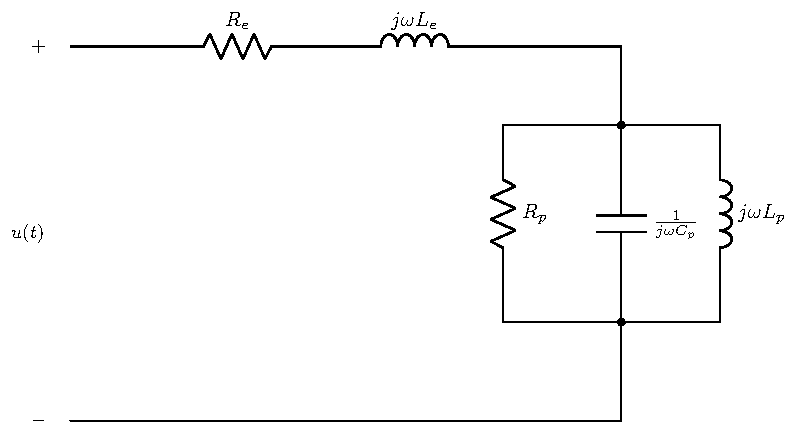
\includegraphics[width=0.4\textwidth]{TU Delft Booming Bass Project Report/figures/FilterGroup/impedance_model_phasor.pdf}
    \captionsetup{justification=raggedright, labelfont=bf}
    \caption{model circuit is phasor domain}
    \label{fig:/model_phasor}
\end{figure}


\section{Loudspeaker simulation}
Using the formulas derived from the circuit model, the corresponding component values can be found for each of the speakers. The calculations were done for each speaker by their respective filter group, which resulted in the component values found in Tab. \ref{tab:speaker_components}. 

Using the parameters found, the frequency response of each model was calculated and compared with the measured speaker data. This showed that the model matched closely around the resonance peak, but that the model generally had a slightly lower impedance than the measured data had as seen in Fig.\ref{fig:/model vs measured impedance}. 

\begin{figure}[H]
    \centering
    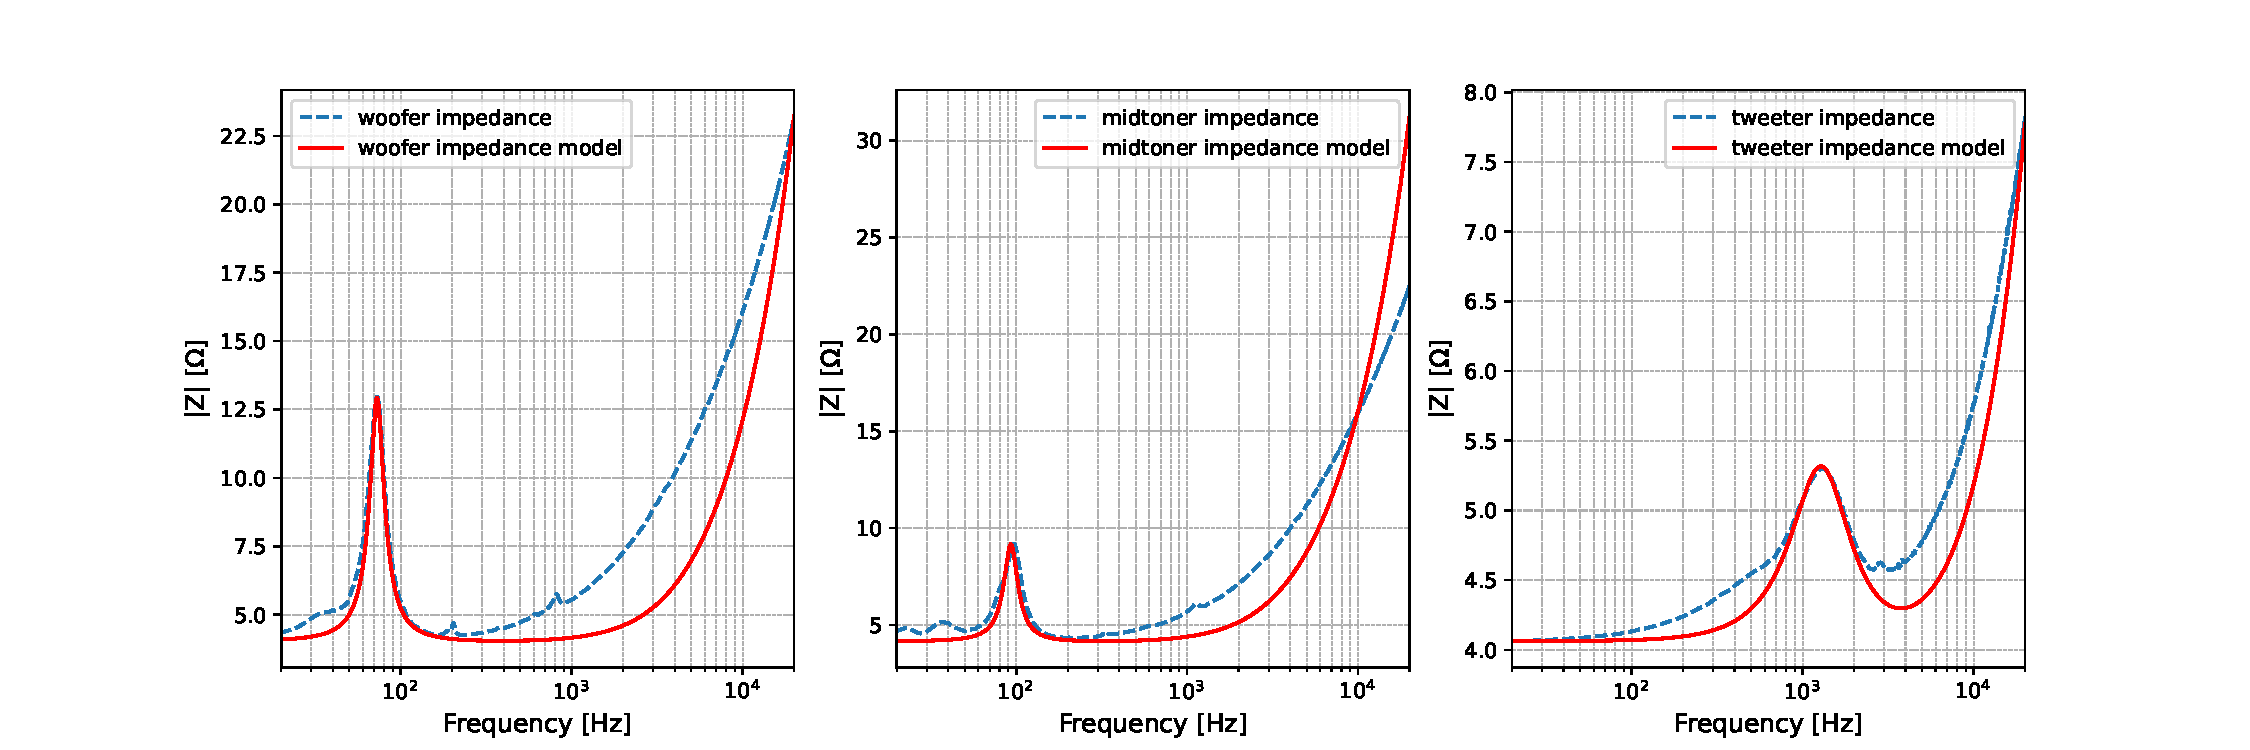
\includegraphics[width=1\textwidth]{TU Delft Booming Bass Project Report/figures/FilterGroup/model vs measured impedance.pdf}
    \captionsetup{justification=raggedright, labelfont=bf}
    \caption{Model speaker impedance versus measured speaker impedance}
    \label{fig:/model vs measured impedance}
\end{figure}

\section{Discussion}
Although the model matches the general shape of the impedance frequency behaviour of the physical circuit, there are still some discrepancies. The most significant of which is that the tweeter's model seems to be the least accurate of the three. This could probably be explained by the fact that the model is better suited for speakers with a lower resonant frequency. Also, at frequencies below and above the resonance peak, the model underestimates the impedance of all three speakers, most greatly for the tweeter.
However, the model does very accurately predict the impedance behavior of the speakers around their resonance peaks, which is the part where the speakers will do most of their work. So, it is most important that the model accurately describes these frequencies. 

\section{Conclusion}
The model of the speaker is an important of the design process as it allows simulations to be done using the model and thusly making the design process a lot simpler. Although the model doesn't match perfectly at every frequency, around the resonance peak it is quite accurate. 